\chapter{Memory Circuits}
\label{ch:memory}

A large part of every GPU's silicon is memory: register files, caches, shared memory. Off the chip sit gigabytes of DRAM. Flip-flops (Chapter~\ref{ch:latch}) are far too big to store that much, so memories use specialized, tiny storage cells packed into dense arrays. This chapter explains the two workhorse cells, SRAM and DRAM, and the circuits around them.

\section{Kinds of memory}

\begin{center}
\small
\begin{tabularx}{\linewidth}{>{\raggedright\arraybackslash}p{2.6cm}*{4}{>{\raggedright\arraybackslash}X}}
\toprule
 & Flip-flop & SRAM & DRAM & Flash \\
\midrule
Cell & 20+ transistors & 6 transistors & 1 transistor, 1 capacitor & 1 special transistor \\
Speed & fastest & very fast & medium & slow (writes very slow) \\
Density & lowest & low & high & highest \\
Needs refresh & no & no & yes & no \\
Keeps data without power & no & no & no & yes \\
Typical use & pipeline registers & caches, register files & main and GPU memory & SSDs, storage \\
\bottomrule
\end{tabularx}
\end{center}

Memory that loses its contents without power is \term{volatile} (SRAM, DRAM); memory that keeps them is \term{nonvolatile} (flash).

\section{How a memory array is organized}

Memory cells are arranged in a grid (Figure~\ref{fig:array}):
\begin{itemize}
  \item Each \textbf{row} shares a horizontal \term{wordline}. Turning a wordline on connects every cell in that row to its column.
  \item Each \textbf{column} shares a vertical \term{bitline} (in SRAM, a pair: $BL$ and $\nt{BL}$), which carries data in and out.
  \item A \term{row decoder} turns the row part of the address into one active wordline (Chapter~\ref{ch:comb}).
  \item \term{Sense amplifiers} at the bottom of the columns detect the small signals the cells put on the bitlines; a \term{column multiplexer} picks which columns are the requested word.
\end{itemize}

\begin{figure}[h]
\centering
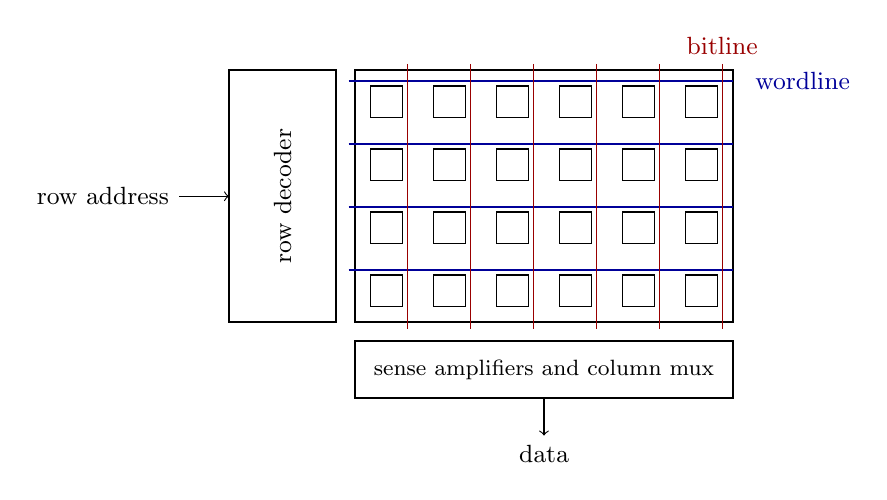
\begin{tikzpicture}[scale=0.8]
  \draw[thick] (0,0) rectangle (6,4);
  \foreach \x in {0.5,1.5,...,5.5} \foreach \y in {0.5,1.5,...,3.5} \draw (\x-0.25,\y-0.25) rectangle (\x+0.25,\y+0.25);
  \foreach \y in {0.5,1.5,...,3.5} \draw[blue!60!black] (-0.1,\y+0.33) -- (6,\y+0.33);
  \foreach \x in {0.5,1.5,...,5.5} \draw[red!60!black] (\x+0.33,4.1) -- (\x+0.33,-0.1);
  \draw[thick] (-2,0) rectangle (-0.3,4); \node[rotate=90,align=center,font=\small] at (-1.15,2) {row decoder};
  \draw[thick] (0,-1.2) rectangle (6,-0.3); \node[font=\footnotesize] at (3,-0.75) {sense amplifiers and column mux};
  \draw[<-] (-2,2) -- (-2.8,2) node[left,font=\small]{row address};
  \draw[->] (3,-1.2) -- (3,-1.8) node[below,font=\small]{data};
  \node[blue!60!black,font=\small,anchor=west] at (6.2,3.83) {wordline};
  \node[red!60!black,font=\small,anchor=south] at (5.83,4.1) {bitline};
\end{tikzpicture}
\caption{A memory array: wordlines select a row; bitlines carry data to the sense amplifiers.}
\label{fig:array}
\end{figure}

\begin{worked}{address bits}
A 256\,Kb ($2^{18}$ bits) SRAM array has 512 rows. Each row then holds $2^{18}/2^9 = 512$ bits. If a word is 32 bits, each row holds 16 words. The address needs $\log_2 512 = 9$ row bits and $\log_2 16 = 4$ column bits: 13 bits to choose one of $2^{13} = 8192$ words.
\end{worked}

\section{The 6T SRAM cell}

An SRAM (static RAM) cell is a bistable loop of two cross-coupled inverters (four transistors) plus two NMOS \term{access transistors} that connect the loop's two nodes to the bitlines when the wordline is high (Figure~\ref{fig:sram}).

\begin{figure}[h]
\centering
\begin{circuitikz}
  \draw (0,0.8) node[not port](i1){};
  \draw (0,-0.8) node[not port, xscale=-1](i2){};
  \draw (i1.out) -- ++(0.4,0) coordinate(r1) -- (r1 |- i2.in) -- (i2.in);
  \draw (i2.out) -- ++(-0.4,0) coordinate(l1) -- (l1 |- i1.in) -- (i1.in);
  \coordinate (qn) at (l1 |- 0,0);
  \coordinate (qbn) at (r1 |- 0,0);
  \fill (qn) circle (0.05); \fill (qbn) circle (0.05);
  \draw (qn) -- ++(-0.6,0) node[nmos, rotate=90, anchor=S](ma){};
  \draw (qbn) -- ++(0.6,0) node[nmos, rotate=90, anchor=D](mb){};
  \draw (ma.D) -- ++(-0.5,0) coordinate(bl);
  \draw (mb.S) -- ++(0.5,0) coordinate(blb);
  \draw (bl |- 0,2.0) node[above]{$BL$} -- (bl |- 0,-2.4);
  \draw (blb |- 0,2.0) node[above]{$\nt{BL}$} -- (blb |- 0,-2.4);
  \draw (ma.G) -- (ma.G |- 0,-1.9);
  \draw (mb.G) -- (mb.G |- 0,-1.9);
  \draw[blue!60!black] ($(bl |- 0,-1.9)+(-0.6,0)$) node[left]{$WL$} -- ($(blb |- 0,-1.9)+(0.6,0)$);
  \node[font=\small,above left] at (qn) {$Q$};
  \node[font=\small,above right] at (qbn) {$\nt{Q}$};
\end{circuitikz}
\caption{A 6T SRAM cell: two cross-coupled inverters store $Q$ and $\nt{Q}$; two access transistors connect them to the bitlines when the wordline $WL$ is high.}
\label{fig:sram}
\end{figure}

\paragraph{Holding.} With the wordline off, the access transistors are off and the loop holds its value indefinitely, as long as power is on. No refresh is needed, which is what ``static'' means.

\paragraph{Reading.} Both bitlines are first \term{precharged} to $\VDD$. Then the wordline turns on. Suppose $Q = 0$. Node $Q$'s side now has a path from the precharged bitline $BL$, through the access transistor and the inverter's pull-down NMOS, to ground, so $BL$ starts to discharge. The other bitline stays high. A sense amplifier detects which bitline is falling, long before it has fallen far.

\paragraph{Read stability.} During that read, node $Q$ (supposed to be 0) is caught in a tug-of-war: the access transistor pulls it up toward the precharged bitline, while the pull-down NMOS pulls it to ground. It is a voltage divider (Chapter~\ref{ch:electricity}), so $Q$ rises a little. If it rises above the other inverter's switching threshold, the cell flips and the read destroys the data (a \term{read upset}). To prevent this, \textbf{the pull-down NMOS must be stronger than the access NMOS}. Their strength ratio is the \term{cell ratio}, typically 1.5 to 2.5.

\paragraph{Writing.} To write $Q = 0$, drive $BL$ to 0 and $\nt{BL}$ to $\VDD$, then turn on the wordline. The access transistor on the $Q$ side must pull $Q$ down \emph{against} the pull-up PMOS that is holding it at 1. So \textbf{the access NMOS must be stronger than the pull-up PMOS} (the \term{pull-up ratio}). Conveniently, PMOS transistors are naturally weaker.

\begin{bigidea}
SRAM cell sizing is a balance: pull-down NMOS $>$ access NMOS $>$ pull-up PMOS. A strong access transistor makes writing easy but reading risky; a weak one makes reading safe but writing hard.
\end{bigidea}

The cell's robustness is measured by its \term{static noise margin} (SNM), read from a plot of the two inverters' transfer curves (the ``butterfly curve''). Process variation (Chapter~\ref{ch:pvt}) makes some cells much weaker than others, which sets the lowest voltage a memory can run at, its $V_{min}$. Some designs use an \textbf{8T cell} with a separate read port that never disturbs the storage nodes, removing the read-stability problem at the cost of area.

\section{Sense amplifiers}

A bitline connects to hundreds of cells, so it has a large capacitance, while each cell's transistors are tiny. Waiting for a cell to swing a bitline all the way to 0 would be very slow. Instead, a \term{sense amplifier} detects a small difference between $BL$ and $\nt{BL}$, often around 100\,mV, and amplifies it to a full logic level. A common design is itself a pair of cross-coupled inverters: released when the bitlines are slightly apart, it quickly regenerates the difference into a full 0 and 1.

\section{DRAM}

A \term{DRAM} (dynamic RAM) cell is one transistor and one capacitor (1T1C). The bit is stored as charge on the capacitor: charged means 1, empty means 0. This is far smaller than an SRAM cell, which is why DRAM provides gigabytes cheaply.

\paragraph{Reading by charge sharing.} The bitline is precharged to $\VDD/2$. Turning on the wordline connects the cell capacitor $C_s$ to the much larger bitline capacitance $C_{BL}$. Charge redistributes, and the bitline moves slightly up (if the cell held a 1) or down (if it held a 0):
\[
  \Delta V = \left(V_{cell} - \frac{\VDD}{2}\right)\frac{C_s}{C_s + C_{BL}}.
\]

\begin{worked}{how big is a DRAM read signal?}
$C_s = 20$\,fF, $C_{BL} = 80$\,fF, $\VDD = 1.2$\,V, and the cell holds a 1 (1.2\,V). The bitline starts at 0.6\,V.
\[
  \Delta V = (1.2 - 0.6) \times \frac{20}{20 + 80} = 0.6 \times 0.2 = 0.12~\text{V}.
\]
Only 120\,mV, which a sense amplifier must detect.
\end{worked}

\paragraph{Destructive reads.} Charge sharing disturbs the cell's own charge, so every read destroys the stored value. The sense amplifier, once it has decided, drives the bitline to a full level, which writes the value back into the cell.

\paragraph{Refresh.} The capacitor slowly leaks its charge. Every cell must be read and rewritten periodically, typically every 64\,ms, which is called \term{refresh}. Refresh costs power and briefly blocks access. That periodic refresh is what ``dynamic'' means.

\paragraph{DRAM organization.} A DRAM chip is divided into \term{banks}. Accessing data first opens a whole row into a \term{row buffer} (slow), after which columns from that open row can be read quickly. Accesses that hit an already open row are much faster than those that need a new row. Graphics memory (GDDR) and high-bandwidth memory (HBM, stacks of DRAM dies next to the GPU) are DRAM organized for very high bandwidth (Chapter~\ref{ch:wires}).

\section{Flash memory}

A \term{flash} cell is a transistor with an extra, electrically isolated gate (a floating gate or a charge-trapping layer) under its control gate. Electrons forced onto that layer by tunneling at high voltage stay there for years without power and shift the transistor's threshold voltage. Reading measures the threshold. Flash is nonvolatile and very dense (cells can store 2, 3 or 4 bits by distinguishing several threshold levels), but writing is slow, it must be erased in large blocks, and each cell survives only a limited number of write cycles. It is used for storage (SSDs), not as working memory.

\section{Register files, CAMs and ROMs}

\begin{itemize}
  \item A \term{register file} is a small, very fast SRAM with many \term{ports}, so several registers can be read and written in the same cycle. Each extra port adds wordlines, bitlines and access transistors to every cell, so ports are expensive. GPUs have very large register files to hold the state of thousands of threads (Chapter~\ref{ch:gpu}).
  \item A \term{content-addressable memory} (CAM) works backwards: you give it a value and it reports which entries contain it, comparing all entries in parallel. CAMs are used in translation lookaside buffers and network routers. They are fast but power-hungry.
  \item A \term{read-only memory} (ROM) holds fixed contents set at manufacture.
\end{itemize}

\section{Protecting stored data: ECC}

Soft errors (Chapter~\ref{ch:fab}) can flip stored bits. A single \term{parity} bit (the XOR of all data bits) detects any single-bit error but cannot say which bit flipped. \term{Error-correcting codes} add more check bits. The common SECDED code (single-error correct, double-error detect) protects 64 data bits with 8 check bits, which is why server and GPU memory often has 72-bit-wide words. Memories may also \term{scrub}: periodically read, correct and rewrite every word so errors do not accumulate.

\section{Summary}

\begin{itemize}
  \item Memory arrays: wordlines select rows, bitlines carry data, decoders select rows, sense amps detect small signals.
  \item 6T SRAM: two cross-coupled inverters plus two access NMOS. Static: no refresh.
  \item Read stability needs pull-down $>$ access; writability needs access $>$ pull-up.
  \item Sense amplifiers turn ~100\,mV bitline differences into full logic levels.
  \item DRAM: 1T1C, read by charge sharing ($\Delta V = (V_{cell} - \VDD/2)\,C_s/(C_s + C_{BL})$), destructive reads, refresh every ~64\,ms.
  \item Flash: nonvolatile, dense, slow to write, limited endurance.
  \item Parity detects single errors; SECDED ECC (64 + 8 bits) corrects them.
\end{itemize}

\section{Exercises}

\begin{enumerate}
  \item How many transistors are in a standard SRAM cell? What are they?
  \item For read stability, which must be stronger: the pull-down NMOS or the access NMOS? Why?
  \item For writability, which must be stronger: the access NMOS or the pull-up PMOS?
  \item A DRAM cell of 30\,fF holding a 1 (1.0\,V) is read onto a 120\,fF bitline precharged to 0.5\,V. Find the bitline change.
  \item Why does DRAM need refresh? Why does SRAM not?
  \item Is a DRAM read destructive? An SRAM read?
  \item A 256\,Kb array has 512 rows and 32-bit words. How many row and column address bits are needed?
  \item How many check bits does SECDED use for 64 data bits?
  \item Why are sense amplifiers needed instead of waiting for full bitline swings?
  \item Which memory keeps its data with power off: SRAM, DRAM or flash?
\end{enumerate}

\subsection*{Answers}
\begin{enumerate}
  \item Six: two PMOS pull-ups and two NMOS pull-downs forming two cross-coupled inverters, plus two NMOS access transistors.
  \item The pull-down. During a read, the 0 node is a voltage divider between them; a stronger pull-down keeps the node low enough that the cell does not flip.
  \item The access NMOS, so it can overpower the PMOS holding the node at 1.
  \item $(1.0 - 0.5) \times 30/150 = 0.1$\,V.
  \item The DRAM capacitor leaks its charge over time. SRAM's cross-coupled inverters actively hold the value from the supply.
  \item DRAM: yes (charge sharing disturbs the cell; it is written back). SRAM: no (if correctly sized).
  \item $2^{18}/512 = 512$ bits per row, so 16 words per row: 9 row bits and 4 column bits.
  \item 8.
  \item Bitlines have large capacitance and cells are tiny, so a full swing would take far too long; sensing a ~100\,mV difference is much faster.
  \item Flash.
\end{enumerate}
